\documentclass[12pt,letterpaper]{article}
\usepackage[utf8]{inputenc}
\usepackage{amsmath}
\usepackage{amsfonts}
\usepackage{amssymb}
\usepackage{booktabs}
\usepackage{hyperref}
\usepackage{tabularx}
\usepackage{graphicx}
\usepackage[normalem]{ulem}
\usepackage{soul}
\usepackage{cancel}
\usepackage{mdframed}
\usepackage{indentfirst}
\usepackage{float}
\usepackage{underscore}
\newmdenv[linecolor=black]{reqbox}

\title{SE 3XA3: Systems Requirements Specification: Revision 0} 
\author{Team 03, Pongthusiastics 		
\\ Adwity Sharma - sharma78 		
\\ Arfa Butt - buttaa3 	
\\ Jie Luo - luoj3 }
 \date{\today} 


\begin{document}
\maketitle
\newpage
\tableofcontents

\listoftables
\listoffigures
\begin{table}[h]
\caption{\bf Revision History}
\begin{tabularx}{\textwidth}{p{3.5cm}p{2cm}X}
\toprule {\bf Date} & {\bf Version} & {\bf Notes}\\
\midrule
October 7, 2016 & 1.0 & Created the SRS document \\
October 11, 2016 & 1.1 & Completed SRS Rev-0 for deadline submission\\
October 24, 2016 & 1.2 & Uploaded diagrams \\
October 31, 2016 & 1.3 & Updated requirements \\
December 7, 2016 & 1.4 & Updated document for Revision 1\\

\bottomrule
\end{tabularx}
\end{table}

\newpage


	
	\section{Project Drivers}
	\subsection{The Purpose of the Project}
	We have overtaken this project to improve the electronic version of ping pong game we found in an open source \textcolor{red}{project on the Git website}. The use of \textcolor{red}{computers and other electronic devices} for entertainment has been growing for several years now. The electronic version of the ping pong game used to be automatically installed with the installation of new windows. But for some years now Microsoft has stopped adding this game to the windows operating system. While, there are variations of this game available for download in the \textcolor{red}{App} store, there is still a market for \textcolor{red}{new and improved ping pong games. Our game} provides the players with a slightly challenging game that does not require any tools other than a computer that has a \textcolor{red}{Java} running environment. This game can be played among friends to relieve themselves of boredom. This project will also provide the users with a game that can be played by people of any age group. \\

	
	\subsection{The Stakeholders}
	\subsubsection{The Client}
	An external entity is regarded the client for this project. This entity is interested in the redevelopment of the project. Though this project is very open ended and can be \textcolor{red}{further} developed in endless manners, there still are some restrictions that \textcolor{red}{have} been applied on the manner of development. This restrictions, in regards to the development has been applied by the 3XA3 team\textcolor{red}{ (3XA3 team defined in Table 2 of Section 1.4)}, and thus can be looked upon as the client figure.\\
			
	\subsubsection{The Customers}
	Any person with an access to a computer that has a \textcolor{red}{Java} running environment can be considered as a customer for this project. As this game does not have restrictions in terms of age, gender or any other socio-economic factor, everyone can be considered as the customer of this project.\\

	\subsubsection{Other Stakeholders}
	We are also the stakeholders for this project, as the development of this project and its result would be a great effect upon us. The general public can also be considered as the stakeholders as through them we are to gain customer base for our game. \textcolor{red}{The rules and regulations of the redevelopment process have been set by the professor and the TAs, so they are also considered as stakeholders.}
	
	\subsection{Mandated Constraints}
	\begin{itemize}
	\item \textbf{Description:} The project is being developed in \textcolor{red}{Java} language in \textcolor{red}{Eclipse} and \textcolor{red}{has to be run in a Java running environment}.\\	
	\textbf{Rationale:} Java running environments such as \textcolor{red}{Eclipse} are available online for free for users and thus can be downloaded by any user intending to play the game.\\	
	\textbf{Fit Criterion:} There shall be a link provided with the release of this game to download a \textcolor{red}{Java} running environment, for users that do not have it already.\\
	\item\textbf{Description:} The project is provided online, in an open source environment, for anyone who wants to use it. Internet connection would be required to download the game the first time \textcolor{red}{the player uses it}.\\	
	\textbf{Rationale:} The user should be connected to the internet that can assure the downloading of the game.\\	
	\textbf{Fit Criterion:} As the game only needs to be downloaded once for the user, it isn’t very hard to accomplish. It only needs to be downloaded once and can be enjoyed for as long as the user intends to use it.
\end{itemize}	

\subsection{Naming Conventions and Terminology}
\begin{table}[H]
\caption{\bf Naming Conventions and Terminology}
\begin{tabular}{|p{3cm}|p{8cm}|}
\hline
\textbf{Terms}    & \textbf{Definitions}                                                                                                                                                                                                                                                                                                                                                                                                                                \\\hline
Users				&	Players of the game \\\hline
The Project 			&	The pong game that is being reconstructed. \\\hline
Product			&	The game that is being developed. \\\hline
Java				&	Java programming language. \\\hline
Clients			& 	The group for whom who the project is being developed for. \\\hline
Git				&	The GitLab website. \\\hline
Windows       		&	Microsoft windows. \\\hline
Customer			&	Anyone who would like to use this game. \\\hline
3XA3 team			&	Professor, course coordinators, teaching assistant and any other personnel responsible for running of the 3XA3 course. \\\hline
Single Player mode		&	The original ping pong game with all the rules from the original project.	\\\hline
Advanced Player mode	&	A new mode with a bomb added to the game.	\\\hline
Bomb				&	Red-colored ball that is to be avoided by the players when playing Advanced mode.	\\\hline
Game scene			&	The window with the game and in-game options.	\\\hline
\end{tabular}
\end{table}

	\subsection{Relevant Facts and Assumptions}
	\textbf{Facts:} There will be approximately 1000 lines of codes for this game by the time this game is completed. The original \textcolor{red}{code} of the game that is being reconstructed can be found in https://github.com/mihneadb/Pong.\\  

	\textbf{Assumptions:} It is assumed that the user will have some access to the internet to download the codes that will be used to run this game when the user wishes to play this game for the first time. It is also assumed that the person will either have access to a \textcolor{red}{Java} running environment or be willing to download a \textcolor{red}{Java} running environment. Since internet is readily accessible this should not be much of a trifle.

	
	\section{Functional Requirements}

	\subsection{The Scope of the Work and the Product}
The developers would rewrite the code into a structured design. By doing this, the work for future maintenance would be easier.

\begin{figure}[h]
  \includegraphics[scale=0.7]{ContextDiagram.png}
  \caption{Context Diagram for the Game}
\end{figure}

	\subsubsection{The Context of the Work}
The software application to be developed will follow the same game rules as the original Pong game application\textcolor{red}{, with the exception of the bomb mode. Bomb mode will have a second red-coloured ball; a bomb, which the players have to miss while not missing the original black ball at the same time.} The interface of the new application would \textcolor{red}{also be improved. There will be additional features added through an in-game options panel. Additionally, the player will be given lives so that there will be a specific termination to the game. Along with the lives, at the end of each game, the player will also be notified of the amount of time they have played.}
	\subsubsection{Work Partitioning}
	The Pong project will be following a model similar to the Water Flow development process. The project will start with developing a problem statement for the new project. It can help team-mates clarify the objective of the work, such as what to improve on the Pong game, and how much we can improve. Team-mates then would like to create a development plan for the Pong game, to make sure each development process is on track and on time. A requirement specification plan is then created to further break down the project into smaller tasks. This include specifying the requirements for the new software, stating the personnel that is related to this Pong project, and clarifying any concerns and issue related to it. A Verification and Validation Plan would be created in the following, to give team members and other stakeholders a vague idea of what the final product would be. Design Specification Document would be formulated for better clarifications before application implementation. Team-mates would be coding following all the documents mentioned, and the Verification and Validation Plan will test the program when it is completed.\\

	The team of three will be working on the redevelopment of the project. Each team member will be assigned different tasks to work on the project. A Gantt Chart will be used to keep track of working activities for each member in the team, that means each member would have to make a mark on the Gantt Chart when they complete a task. \\

\begin{figure}[h]
  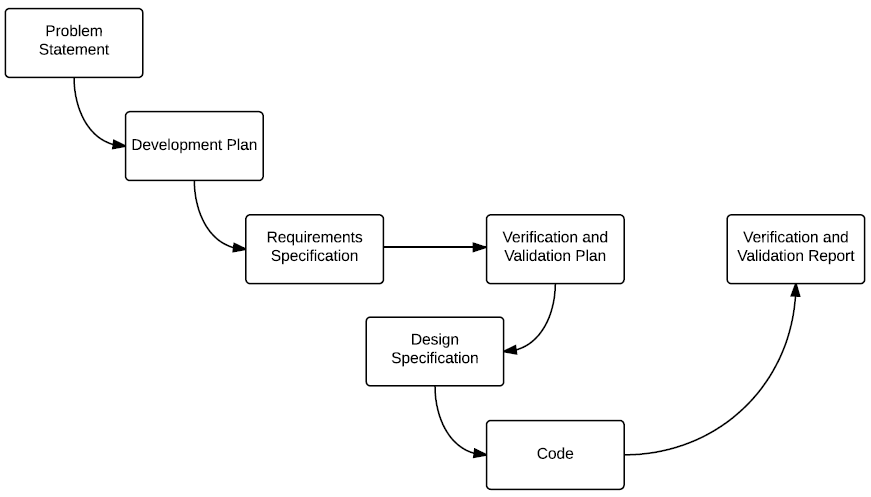
\includegraphics[scale=0.6]{ProjectFlow.png}
  \caption{Project Flow for the Redevelopment Process}
\end{figure}

\subsubsection{Individual Product Use Cases}
\begin{itemize}

	\item Case: User performs mouse click on the \textcolor{red}{Start New Game} button\\
	Result: The program would \textcolor{red}{show the New Game page with the option to start a Single Player mode or an Advanced Player mode}.\\

	\item \textcolor{red}{Case: User performs mouse click on Single Player Mode button}\\
	\textcolor{red}{Result: The program would start a Single Player mode game and the game scene would be displayed.}\\

	\item \textcolor{red}{Case: User performs mouse click on Advanced Player Mode button}\\
	\textcolor{red}{Result: The program would start an Advanced Player mode game and the game scene would be displayed.}\\
	
	\item Case: User performs mouse click on the Save Game button\\
	Result:  The program would save the players’ record, \textcolor{red}{and the game itself would be paused until the user clicks resume.} \\
	
	\item \textcolor{red}{Case: User performs mouse click on Pause Game button}\\
	\textcolor{red}{Result: The program would pause the game.}\\

	\item \textcolor{red}{Case: User performs mouse click on Resume Game button}\\
	\textcolor{red}{Result: The program would resume the game.}\\

	\item \textcolor{red}{Case: User performs mouse click on Exit to Main Page button}\\
	\textcolor{red}{Result: The program would exit the game scene and go back to the Main Page.}\\

	\item Case: User performs mouse click on the \textcolor{red}{Load Game} button\\
	Result: The program would \textcolor{red}{load the previously saved game.}\\

	\item \textcolor{red}{Case: User performs mouse click on High Scores button}\\
	\textcolor{red}{Result: The program would display the top MAX_HS number of highscores.}\\

	\item Case: User performs mouse click on the Tutorial button\\
	Result: The program would display a description of the game and teach the user how to play it.\\

	\item Case: User performs mouse click on the \textcolor{red}{Exit} button\\
	Result: The program game would stop, the window of the application would be closed, and the current game result would not be saved.\\

	\item Case: User taps on \textcolor{red}{ LEFT and RIGHT keys} on the keyboard\\
	Result: The player would be able to move his/her \textcolor{red}{paddle in the game}.\\
\end{itemize}

	\subsection{Functional Requirements}

\begin{reqbox}
	\begin{itemize}
		\textbf{Requirement number: }FR1  
		
		The program should have a button to start a new game.  
		 
		\textbf{Rationale: } The user should be able to start a new game in order to play the game.
		
		\textbf{Priority: }High

		\textbf{History: }Created October 11, 2016
	\end{itemize}
\end{reqbox}

\begin{reqbox}
	\begin{itemize}

		\item \textbf{Requirement number: }FR2  
		
		 The program should have a button to load a previously saved game.

		\textbf{Rationale: }The user must be able to load his/her previously saved game in order to continue the game.

		\textbf{Priority: }High

		\textbf{History: }Created October 11, 2016
	\end{itemize}
\end{reqbox}

\begin{reqbox}
	\begin{itemize}

		\item \textbf{Requirement number: }FR3

		The program should have a button to save the current game.

		\textbf{Rationale: }The user must be able to save their current game in order to continue playing it at a later time.

		\textbf{Priority: }High

		\textbf{History: }Created October 11, 2016

	\end{itemize}
\end{reqbox}

\begin{reqbox}
	\begin{itemize}

		\item \textbf{Requirement number: }FR4

		The program should be able to display a list of top \textcolor{red}{MAX_HS high scores (name and their time)}. 

		\textbf{Rationale: }The user must be able to open up the high scores list, so that they can see what rank they are on. This will also build healthy competition among the players.

		\textbf{Priority: }High

		\textbf{History: }Modified December 7, 2016

	\end{itemize}
\end{reqbox}

\begin{reqbox}
	\begin{itemize}
		\item \textbf{Requirement number: }FR5

		The program should have a button to open up the tutorial page, which will give instructions to the user on how to play the game.

		\textbf{Rationale: }If the user is playing the game for the first time, they must be able to view the instructions to the game before they can play it.

		\textbf{Priority: }Medium

		\textbf{History: }Created October 11, 2016
	\end{itemize}
\end{reqbox}

\begin{reqbox}
	\begin{itemize}

		\item \textbf{Requirement number: }FR6

		The program should have a button to have the option to play a single-player mode, with the computer. The list of high scores will be kept for this mode.

		\textbf{Rationale: }The user must choose which type of mode of the game they want to play, before they can play the game. This type of mode is for users who want to play alone, or want to beat a certain high score.

		\textbf{Priority: }High

		\textbf{History: }Created October 11, 2016

	\end{itemize}
\end{reqbox}

\begin{reqbox}
	\begin{itemize}
		\item \textbf{Requirement number: }FR7

		The program should have a button for the option to play \textcolor{red}{an Advanced player} mode, with the computer. 

		\textbf{Rationale: }The user must choose which type of mode of the game they want to play, before they can play the game. This type of mode is for users who want to play the single-player mode, but with a little added difficulty.

		\textbf{Priority: }Medium

		\textbf{History: }Modified December 7, 2016
	\end{itemize}
\end{reqbox}

\begin{reqbox}
	\begin{itemize}
		\item \textbf{Requirement number: }FR8

		At the start of \textcolor{red}{every} game, the player should have\textcolor{red}{ MAX_LIVES number of}  lives.

		\textbf{Rationale: }The user must have \textcolor{red}{a specific number of} lives at the start of the game, as that is the standard that we have decided to keep for the game.

		\textbf{Priority: }High

		\textbf{History: }Modified December 7, 2016
	\end{itemize}
\end{reqbox}

\begin{reqbox}
	\begin{itemize}
st{
		\item \textbf{Requirement number: }FR9

		At the start of \textcolor{red}{an Advanced player mode, the computer should have MAX_LIVES number of lives}.

		\textbf{Rationale: }\textcolor{red}{The computer must have the same number of lives as the player to keep the game fair.}

		\textbf{Priority: }High

		\textbf{History: }Modified December 7, 2016
}
	\end{itemize}
\end{reqbox}

\begin{reqbox}
	\begin{itemize}
		\item \textbf{Requirement number: }FR10

		The user should be able to move their paddle left and right using the keyboard.

		\textbf{Rationale:} The user must be able to move their paddle left and right in order to play the game.

		\textbf{Priority: }High

		\textbf{History: }Created October 11, 2016
	\end{itemize}
\end{reqbox}

\begin{reqbox}
	\begin{itemize}

		\item \textbf{Requirement number: }FR11

		\textcolor{red}{Whenever a player misses a hit}, their life should be decreased by 1.

		\textbf{Rationale: }The number of lives of each player should decrease by 1 each time the player misses the ball, to keep track of the number of lives the player has left. This is to make sure that the player does not go over MAX_LIVES.

		\textbf{Priority: }High

		\textbf{History: }Modified December 7, 2016
	\end{itemize}
\end{reqbox}

\begin{reqbox}
	\begin{itemize}

		\item \textbf{Requirement number: }FR12

		The program should have a button to pause the current game.

		\textbf{Rationale: }The user must be able to pause the current game so that if they need a short break, they can take one without it affecting the progress of their current game.

		\textbf{Priority: }High

		\textbf{History: }Created October 11, 2016
	\end{itemize}
\end{reqbox}

\begin{reqbox}
	\begin{itemize}
		\item \textbf{Requirement number: }FR13

		The program should have a button to resume the current game (if the game is paused).

		\textbf{Rationale: }The user must be able to resume the current game so that if the game is paused, it can be resumed from the point where the player left the game.

		\textbf{Priority: }High
	
		\textbf{History: }Created October 11, 2016
	\end{itemize}
\end{reqbox}

\begin{reqbox}
	\begin{itemize}
		\item \textbf{Requirement number: }FR14

		The user should have the ability to \textcolor{red}{exit back to the main page without terminating the whole program}.

		\textbf{Rationale: }The user must be able to \textcolor{red}{go back to the main page from the current game so that if they are not satisfied with their game, and would like to play a new game, they may do so by just going back to the main page and starting a new   game}.

		\textbf{Priority: }High

		\textbf{History: }Modified December 7, 2016
	\end{itemize}
\end{reqbox}

\begin{reqbox}
	\begin{itemize}
		\item \textbf{Requirement number: }FR15

		\textcolor{red}{Whenever one player misses the ball MAX_LIVES times, the game should end as that players last lost all of their lives.}

		\textbf{Rationale: }The standard for this game has been set so that each player gets MAX_LIVES lives, therefore the game needs to end once the player has used up all of their lives.

		\textbf{Priority: }High

		\textbf{History: }Modified December 7, 2016
	\end{itemize}
\end{reqbox}

\begin{reqbox}
	\begin{itemize}
		\item \textbf{Requirement number: }FR16
	
		Once a game ends, the user should be taken back to the main menu page.

		\textbf{Rationale: }The user must be taken back to the main menu page so that they can choose which mode of game they want to play, or if they want to access the high scores list.

		\textbf{Priority: }High

		\textbf{History: }Created October 11, 2016
	\end{itemize}
\end{reqbox}

\begin{reqbox}
	\begin{itemize}
		\item \textbf{Requirement number: }FR17

		In single-player mode if the player made it into the high scores list then, at the end of the game before the user is taken back to the main menu, (s)he will be prompted to enter their name so that they could be added into the list.

		\textbf{Rationale: }The user must be prompted for their name if they break one of the high scores, so that the list of high scores is kept up to date.

		\textbf{Priority: }High

		\textbf{History: }Created October 11, 2016
	\end{itemize}
\end{reqbox}

\begin{reqbox}
	\begin{itemize}
		\item \textbf{Requirement number: }FR18

		At the end of the game, a window should pop up to indicate the winning and losing state.

		\textbf{Rationale: }The user need to be notified the end of the game.

		\textbf{Priority: }High

		\textbf{History: }Created October 31, 2016
	\end{itemize}
\end{reqbox}
		

\section{Nonfunctional Requirements}
\subsection{Look and Feel Requirements}

\begin{reqbox}
	\begin{itemize}
	\item \textbf{Requirement number: }NFR1

		The game interface should be colorful and vivid.

		\textbf{Rationale: } The user would be interested in the game if its interface is attractive.

		\textbf{Priority: } \textcolor{red}{Medium}

		\textbf{History: } Modified December 7, 2016
	
		\item \textbf{Requirement number: }NFR2

		The game frame should be clear for user to play.

		\textbf{Rationale: } The user should know where the border of the game frame is, in order to move his/her paddle to the proper prositions

		\textbf{Priority:  }High

		\textbf{History: } Created October 31, 2016

	\end{itemize}
\end{reqbox}


\subsection{Usability and Humanity Requirements}

\begin{reqbox}
	\begin{itemize}
	\subsubsection{Ease of Use Requirements}	

	\item \textbf{Requirement number: }NFR3
	   	
		The game can be played by nighty-nine percents of people who know  how to use a computer with hands.

		\textbf{Rationale: } This game utilizes only mouse and keyboard.

		\textbf{Priority: }High

		\textbf{History: }Modified October 31, 2016

	\end{itemize}
\end{reqbox}

\begin{reqbox}
	\begin{itemize}
 	
 	\item \textbf{Requirement number: }NFR4
 	
   	The game is easy enough to for a child greater than \textcolor{red}{x} years old to play. Some practice on the part of the users might be required to play and excel at this game.

		\textbf{Rationale: } This game should be available for most of the children because the game is focused on the children.

		\textbf{Priority: }High

		\textbf{History: }Modified December 7, 2016

	\end{itemize}
\end{reqbox}

\begin{reqbox}
	\begin{itemize}

 	\subsubsection{Accessibility Requirements}
 	
 	\item \textbf{Requirement number: }NFR5
 	
	The game can be accessed and executed on majority of computing devices. 

		\textbf{Rationale: } Computers with Java installed should be able to open this game. Meanwhile, as long as there is \textcolor{red}{an internet connection, this game is available for download}.

		\textbf{Priority: }High

		\textbf{History: }Modified December 7, 2016
	

	\end{itemize}
\end{reqbox}


\subsection{Performance Requirements}

\begin{reqbox}
	\begin{itemize}
\subsubsection{Speed requirement}

\item \textbf{Requirement number: }NFR6

   	There has to be some space in the user’s computer to download the game and a \textcolor{red}{Java} running environment. The game should be played in a fast computer as it would decrease the entertainment factor if it is lagging.

		\textbf{Rationale: } As long as the computer with this game has enough space for caching for Java, the speed of the game should be fast enough for playing.

		\textbf{Priority: }High

		\textbf{History: }Modified December 7, 2016

	\end{itemize}
\end{reqbox}

\begin{reqbox}
	\begin{itemize}

\subsubsection{Safety critical requirement}

\item \textbf{Requirement number: }NFR7

		The program should be able to finish in reasonable amount of time.  

		\textbf{Rationale: } Over-playing the game might cause the user to encounter some strain in the user’s eyes.\textcolor{red}{ However, this is true for all games that require an electronic screen to play. Other than this, there are no other health concerns.}

		\textbf{Priority: }Medium

		\textbf{History: }Modified December 7, 2016

	\end{itemize}
\end{reqbox}

\begin{reqbox}
	\begin{itemize}

\subsubsection{Precision requirement}

\item \textbf{Requirement number: }NFR8

		The movements of the paddle should be as accurate as \textcolor{red}{the actions performed on the keyboard.}

		\textbf{Rationale: } Actions performed on the keyboard would directly affect player scores and satisfiability of the game.

		\textbf{Priority: }Medium

		\textbf{History: }Modified December 7, 2016

	\end{itemize}
\end{reqbox}

\begin{reqbox}
	\begin{itemize}

\subsubsection{Reliability and availability requirement}

\item \textbf{Requirement number: }NFR9

		The game shall take less than five seconds to start up on 90 percents of computers.

		\textbf{Rationale: } The program does not take up a lot of memory spaces or cache on the computer, so the startup should be rather quick.

		\textbf{Priority: }Medium

		\textbf{History: }Modified October 31, 2016

		\item \textbf{Requirement number: }NFR10	
		
		The program shall take less than two seconds to perform actions after \textcolor{red}{a button is pressed.} 

		\textbf{Rationale: } Similarly, since the program does not take up a lot of memory spaces or cache on the computer, it should not take a long time for responding.

		\textbf{Priority: }Medium

		\textbf{History: }Modified December 7, 2016

	\end{itemize}
\end{reqbox}

\begin{reqbox}
	\begin{itemize}

\subsubsection{Capacity requirement}

\item \textbf{Requirement number: }NFR11

		The game shall not have memory explode due to huge player record storage.

		\textbf{Rationale: } The game records at most MAX_HS player records on a file, therefore, it should not take up much storage on the computer.

		\textbf{Priority: }Medium

		\textbf{History: }Modified December 7, 2016


	\end{itemize}
\end{reqbox}

\subsection{Operational and Environmental Requirements}

\begin{reqbox}
	\begin{itemize}
\subsubsection{Expected Physical Environment}
	\item \textbf{Requirement number: }NFR12

	The application should be able to run on a computer whenever the computer functions properly.

	\textbf{Rationale: }The program should be able to run when the computer is running; otherwise the program would be considered a failure.

	\textbf{Priority: }High
	
	\textbf{History: }Created October 11, 2016
	\end{itemize}
\end{reqbox}

\subsection{Expected Technological Environment}

\begin{reqbox}
	\begin{itemize}
	\item \textbf{Requirement number: }NFR13

	The application should be able to run on any computer with Java version 1.7 or higher installed

	\textbf{Rationale: }The application is developed under Java version 1.7 environment, so the user should be able to run it under the same environment. 

	\textbf{Priority: }High

	\textbf{History: }Created October 11, 2016

	\end{itemize}
\end{reqbox}

\begin{reqbox}
	\begin{itemize}
\subsubsection{Partner Application}

	\item \textbf{Requirement number: }NFR14

	The application should be able to run on any Java IDE with Java version 1.7 or higher

	\textbf{Rationale: }The application is developed on a Java IDE with version 1.7 environment, so the user should be able to run it under the same environment. 

	\textbf{Priority: }High

	\textbf{History: }Created October 11, 2016
	\end{itemize}
\end{reqbox}


\subsection{Maintainability and Support Requirements}

\begin{reqbox}
	\begin{itemize}
\subsubsection{Maintenance Requirement}

	\item \textbf{Requirement number: }NFR15

	The application should be under minimal maintenance.

	\textbf{Rationale: }\textcolor{red}{Most of the bugs that occur during the gaming process should be discovered during or after testing, and should be corrected and fixed.}

	\textbf{Priority: }High

	\textbf{History: }Modified December 7, 2016

	\end{itemize}
\end{reqbox}

\begin{reqbox}
	\begin{itemize}

\subsubsection{Supportability Requirement}

	\item \textbf{Requirement number: }NFR16
	
	 The application should run on the majority of users’ computers.

	\textbf{Rationale: }Most of the potential players should be able to play the Pong game. 
	
	\textbf{Priority: }High    

	\textbf{History: }Created October 11, 2016    

	\end{itemize}
\end{reqbox}

\begin{reqbox}
	\begin{itemize}

\subsubsection{Portability Requirement}
	\item \textbf{Requirement number: }NFR17

	The application should have their file size less than \textcolor{red}{MAX_MB}.

	\textbf{Rationale: }This game should be easy to transfer between users for easy access. Players could use any storage devices to transfer files.

	\textbf{Priority: }High

	\textbf{History: }Modified December 7, 2016
	\end{itemize}
\end{reqbox}

\subsection{Security Requirements}

\begin{reqbox}
	\begin{itemize}
\subsubsection{Confidentiality}
None applicable to this project.
	\end{itemize}
\end{reqbox}

\begin{reqbox}
	\begin{itemize}

\subsubsection{File Integrity Requirement}

	\item \textbf{Requirement number: }NFR18  
	
	The files for the application should have the extension .JAVA.

	\textbf{Rationale: }Files need to be recognized as \textcolor{red}{Java} files before executions.
	
	\textbf{Priority: }High     
	 
	\textbf{History: }Created October 11, 2016  
	\end{itemize}
\end{reqbox}

\begin{reqbox}
	\begin{itemize}

\subsubsection{Audit Requirement}
None applicable to this project.

	\end{itemize}
\end{reqbox}

\subsection{Cultural Requirements}

\begin{reqbox}
	\begin{itemize}
	\item \textbf{Requirement number: }NFR19 
	
	The language that shall be used in this game is English.

	\textbf{Rationale: }English is the language that all students and faculty members of McMaster University are expected to understand.

	\textbf{Priority: }High
	
	\textbf{History: }Created October 11, 2016
	\end{itemize}
\end{reqbox}

\begin{reqbox}
	\begin{itemize}
	\item \textbf{Requirement number: }NFR20

	The program shall not contain any imagery or language that can be viewed as offensive to users by mocking, insulting, or appropriating their culture, race, or religion.

	\textbf{Rationale: }User satisfaction will be affected if the material and contents of this game are perceived as offensive to the consumers.

	\textbf{Priority: }Medium

	\textbf{History: }Created October 11, 2016
	\end{itemize}
\end{reqbox}

\subsection{Legal Requirements}

\begin{reqbox}
	\begin{itemize}

	\item \textbf{Requirement number: }NFR21   
	
	The program will adhere to the MIT Open License.

	\textbf{Rationale: }The program will adhere to the MIT License as it is the standard that is set for this project.
	
	\textbf{Priority: }Medium   
	
	\textbf{History: }Created October 11, 2016   
	\end{itemize}
\end{reqbox}


\section{Project Issues}
\subsection{Open Issues}
So far there aren’t any open issues.
\subsection{Off-the-Shelf Solutions}
The game that this project is attempting to reconstruct would act as an initial model for this project that we have overtaken. There are also other similar games available and the way certain parts are executed can provide a model for us to base our design on. There are also guidance and directions available in \textcolor{red}{Java} tutorial sites for any programming problems that are likely to occur during the development of this game.  
\subsection{New Problems}
\subsubsection{Problems in the Current Environment}
None applicable in the project.
\subsubsection{Existing User}
Is there a way to clear user record?
\subsubsection{Limitations in Implementation Environment} 
Is it possible to run on every device that has Java?
\subsection{Tasks}
Tasks Deadline

Model Development October 14

View Development October 14

Control Development October 17

Project Revision October 31

Project Improvement November 19
\subsection{Migration to the New Product}
None applicable in the project.
\subsection{Risks}
There are no risks associated with this project.
\subsection{User Documentation and Training}
The user documents will be created as per the SE 3XA3 guidelines.
There will be an in-game tutorial that will display the instructions on how to play the game. Other than that, no further training should be required..
\subsection{Waiting Room}
There are many factors in the game that has to be improved upon, as has been discussed throughout various parts in the document. The improvement of functionality of the game is to be looked forward towards. The addition of sound to the game can also be added to this.
\subsection{Ideas for Solutions}
Proper documentations for the game must be made. The coding for the game should be well commented and easy to follow. Other then this, for the current period there isn’t any other ideas for solutions. This section would be updated at a later period. 
\section{Appendix}
\subsection{Symbolic Parameters}
Section 1.4 provides a list of terms and its definition of any symbols that are used throughout the document. \textcolor{red}{Some parameters that are not included in Table 2 are as follows: }
\begin{table}[H]
\caption{\bf Symbolic Parameters}
\begin{tabular}{|p{3cm}|p{10cm}|}
\hline
\textbf{Terms}    & \textbf{Definitions}                                                                                                                                                                                                                                                                                                                                                                                                                                \\\hline
MAX_HS		&	Maximum number of highscores - set to 20 for this project	\\\hline
MAX_LIVES		&	Maximum number of lives given to the user and the computer - set to 3 for this project	\\\hline
x 			&	People above this age can play this game - assumed to be 10	\\\hline
MAX_MB 		&	Maximum storage needed to download/play this game - assumed to be 50MB 	\\\hline
\end{tabular}
\end{table}
\end{document}